\section{Pretraining Process}

The training process begins with the initialization of the ResNet-34
backbone using pre-trained weights, providing a strong foundation for
feature extraction. The model's hyperparameters are optimized using
Optuna \cite{AkibaEtAl2019}, a hyperparameter optimization framework
that employs Bayesian
optimization to search for optimal values of:

\begin{itemize}
  \item Learning rate: Sampled logarithmically between $10^{-6}$
    and $10^{-2}$
  \item TGCE$_{SS}$ parameters:
    \begin{itemize}
      \item $q$: Controls truncation of the loss function (0.1 to 0.9)
      \item Noise tolerance: Controls model's robustness to label
        noise (0.1 to 0.9)
      \item Regularization weights: Control the balance between
        different loss terms.
    \end{itemize}
\end{itemize}

\subsection{Hyperparameter Optimization Pretraining
Study}\label{sec:pretraining-study}

A hyperparameter optimization study was conducted for every single
reliability branch estimation type (scalar, pixel and features) using Optuna,
each with 20 iterations, on the Oxford PET dataset with three scorers
emulating SNR noises of -20, 0, and 10 dB respectively, and a labeling
rate of 0.5.

The analysis of hyperparameter importance reveals crucial insights
about the regularization terms' contributions to model performance.
As shown in Figure~\ref{fig:optuna_study_combined}, the contour plots
visualize the optimization landscape for different regularization
parameters, providing complementary evidence to the importance
scores. Table~\ref{tab:hyperparameter_importance_regularizers} presents the
hyperparameter importance ranking for the regularizers study for each
reliability estimation approach.

The contour visualizations (Figure \ref{fig:optuna_study_combined}) and
importance analysis consistently demonstrate that the sum
regularization ($\alpha_{\text{sum}}$) exhibits the lowest importance
across all reliability estimation approaches, with scores of 0.0756,
0.0661, and 0.0219 for pixel, scalar, and features approaches
respectively. This low importance, combined with the relatively flat
contour regions observed in the optimization landscape, suggests that
the sum regularization's contribution might be largely redundant with
the combination of centroid and entropy regularization terms. This
finding has significant implications for model design: since sum regularization
requires sigmoid activation in the output layer, while centroid and
entropy regularization can work with softmax outputs, eliminating the
sum regularization term allows for the use of fully softmax outputs
in subsequent experiments. This simplification reduces the
hyperparameter search space and potentially improves training
stability, making the optimization process more efficient for future
experiments. This is likely to happen because of the combination of entropy
and centroid regularization terms, which are also related to
controlling homogeneity or extreme reliability values, leading to an
undermining of the sum regularization term, in such scenario, the sum
regularization term would be redundant.

\begin{table}[h]
  \centering
  \begin{tabular}{lccc}
    \toprule
    \multirow{2}{*}{\textbf{Hyperparameter}} &
    \multicolumn{3}{c}{\textbf{Importance Score}} \\
    \cmidrule(lr){2-4}
    & \textbf{Pixel} & \textbf{Scalar} & \textbf{Features} \\
    \midrule
    $\alpha_{\text{sum}}$ & 0.0756 & 0.0661 & 0.0219 \\
    $\alpha_{\text{entropy}}$ & 0.0268 & 0.1342 & 0.5395 \\
    $\alpha_{\lambda}$ & 0.0234 & 0.3362 & 0.0282 \\
    $\beta$ & 0.0200 & 0.2999 & 0.0218 \\
    $a$ & 0.1738 & 0.1636 & 0.3886 \\
    \bottomrule
  \end{tabular}
  \caption{Hyperparameter importance ranking for regularization parameters
    obtained from Optuna optimization study after 20 iterations for each
    reliability estimation approach (pixel, scalar, and features). This study
    used preselected values of $q=0.66$, $\tilde{C}=0.62$, and learning
    rate $=6.5 \times 10^{-4}$. The importance scores indicate the relative
    impact of each regularization hyperparameter on the model's performance
  for each specific approach.}
  \label{tab:hyperparameter_importance_regularizers}
\end{table}

\begin{figure}[h!]
  \centering
  \begin{subfigure}[b]{0.75\textwidth}
    \centering
    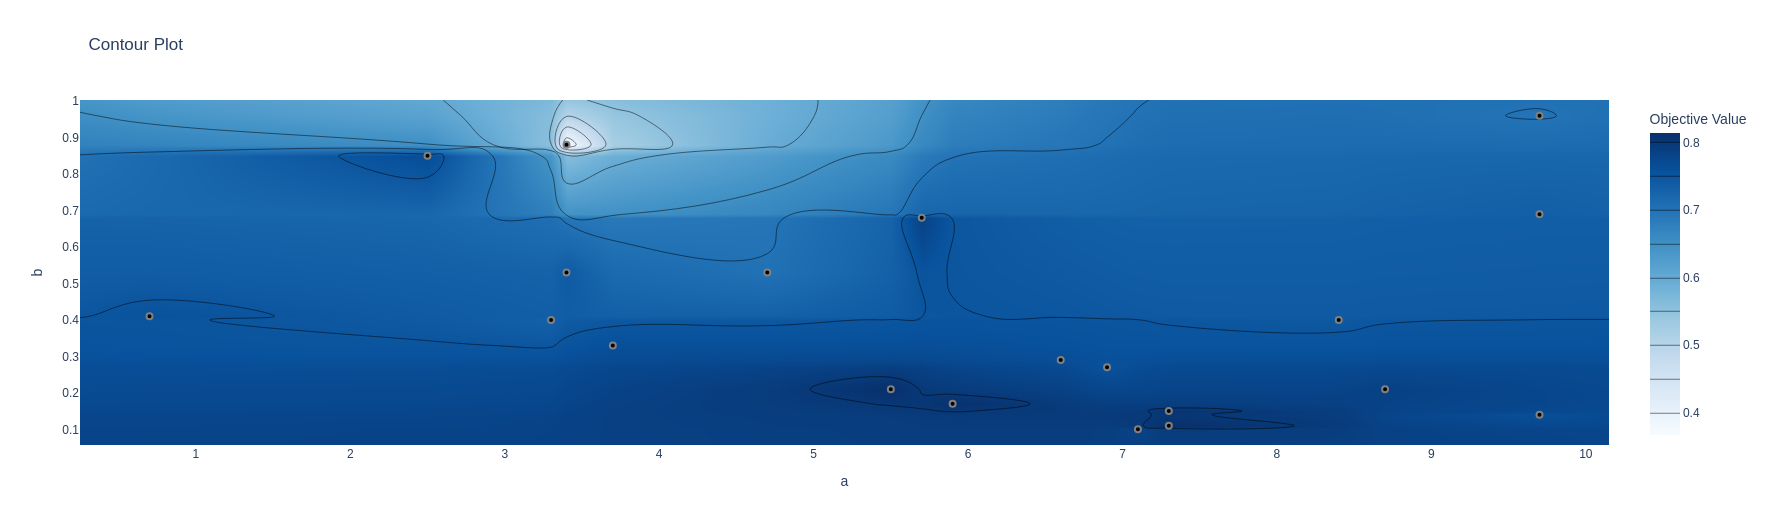
\includegraphics[width=\textwidth]{Cap5/Figures/contours_oxford_features_a_b.png}
    \caption{Missing labels penalty regularization
    ($\alpha_{\lambda}$ and $\beta$).}
    \label{fig:optuna_study_a_b}
  \end{subfigure}
  \hfill
  \begin{subfigure}[b]{0.75\textwidth}
    \centering
    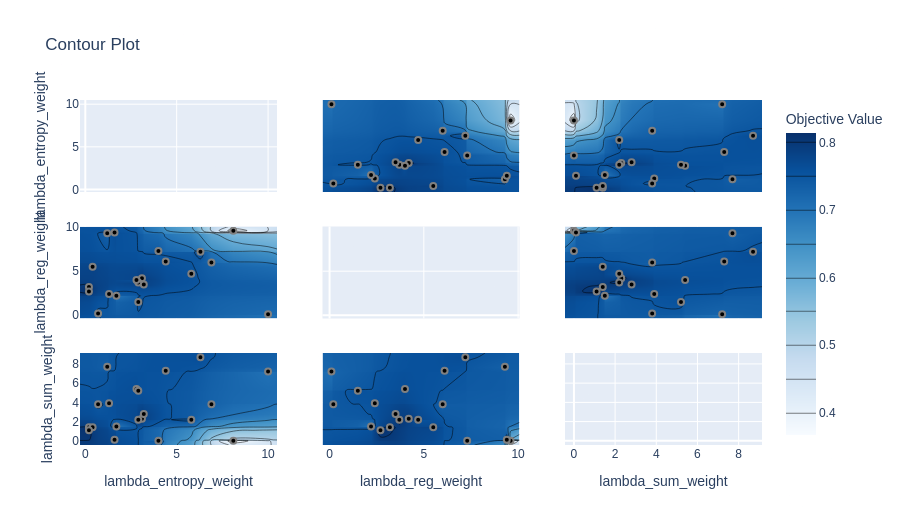
\includegraphics[width=\textwidth]{Cap5/Figures/contours_oxford_features_others.png}
    \caption{Other regularization terms
      ($\alpha_{\text{centroid}}$, $\alpha_{\text{sum}}$,
    $\alpha_{\text{entropy}}$).}
    \label{fig:optuna_study_others}
  \end{subfigure}
  \caption{Contours of the tuner optimization study for the Oxford
    PET dataset with the best hyperparameters found for the
  comprehensive hyperparameter optimization study.}
  \label{fig:optuna_study_combined}
\end{figure}

\subsection{Training Process Overview}

After finding the optimal hyperparameters, the model is trained end-to-end
using the Adam optimizer with the best learning rate found
\footnote{For every experiment this was also tuned with the help of
the Optuna study, having different optimal values for every experiment.}. The
TGCE$_{SS}$ loss function plays a crucial role in updating both the
segmentation and reliability branches, ensuring that the model learns
to effectively handle multiple annotators' inputs while accounting
for their varying reliability.

\begin{figure}[h]
  \centering
  \begin{tikzpicture}[
      node distance=1.2cm and 1.5cm,
      every node/.style={font=\footnotesize},
      box/.style={draw, rectangle, minimum width=2.5cm, minimum
      height=1cm, align=center},
      arrow/.style={-{Latex}, thick},
      roundedbox/.style={draw, rectangle, rounded corners=5pt,
      minimum width=4.2cm, minimum height=1.2cm, align=center}
    ]

    % Dataset notation
    \node[align=left] (dataset) at (-4.5,1.5) {
      \textbf{Train Dataset} \\
      $\left\{(x_n, \tilde{y}^r_n)\right\}_{r \in R_n}^{n \in \mathbb{N}}$
    };

    % Image box
    \node[box, right=2cm of dataset] (image) {%
      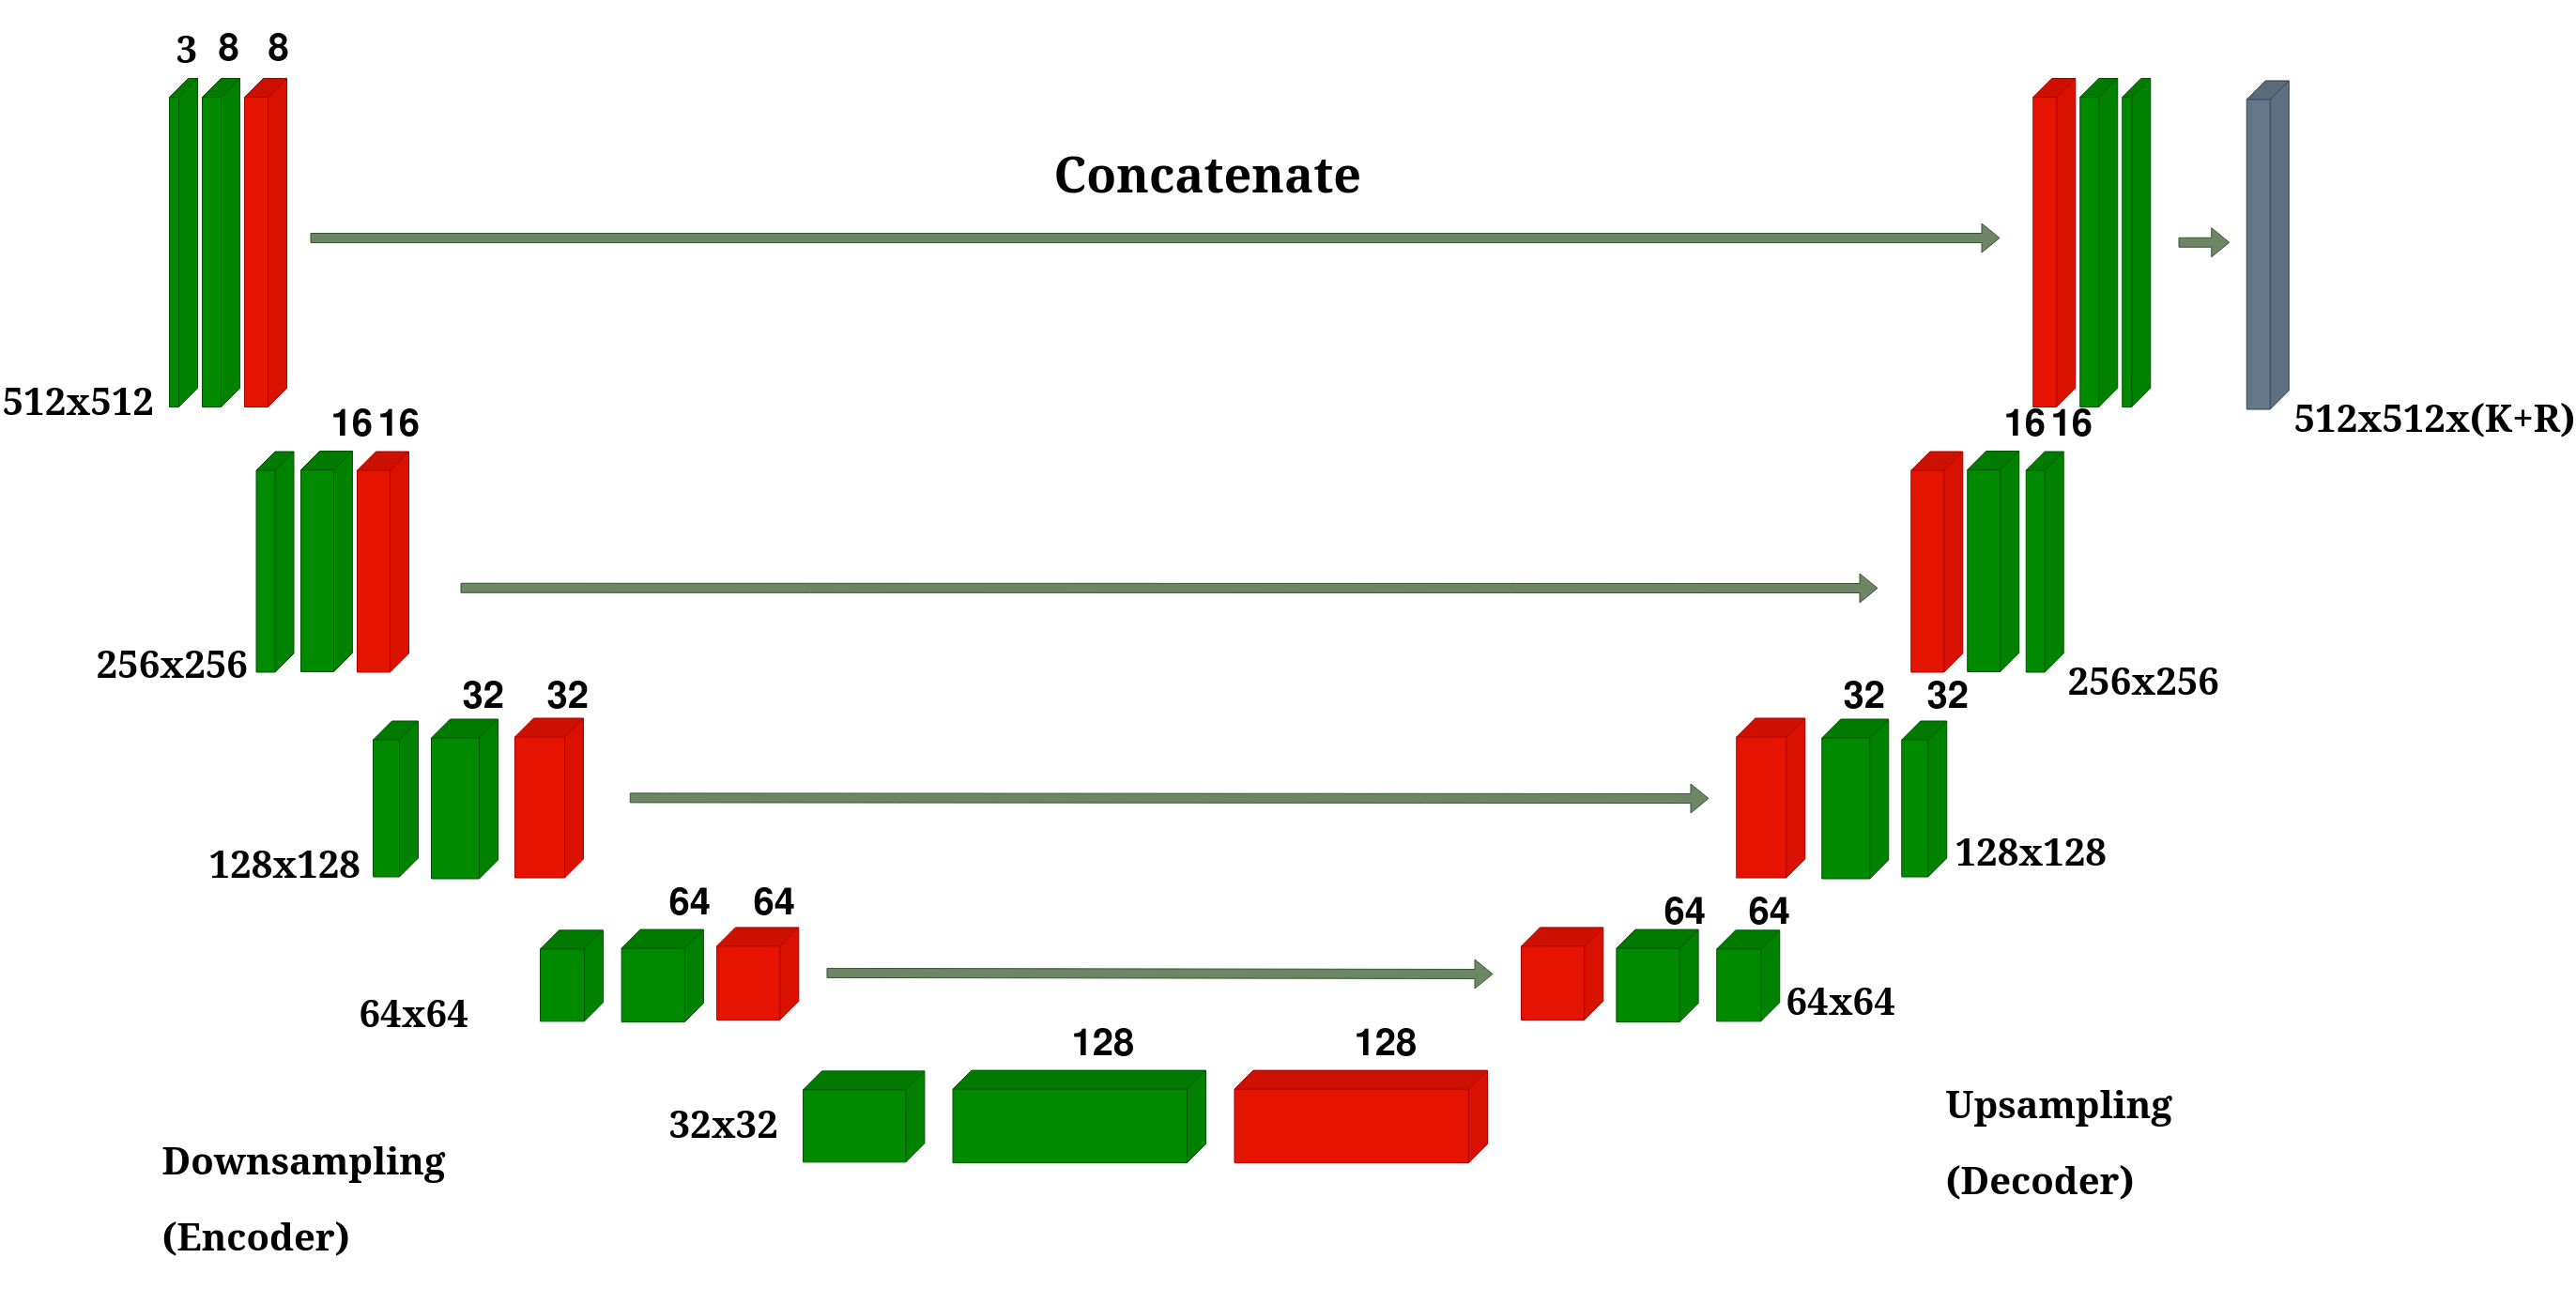
\includegraphics[width=2.5cm]{Cap5/Figures/cnn_arch_overview.png}
    };

    % Output of model
    \node[align=left, right=of image] (modelout) {
      $\left[ f(x; \theta), \; \Lambda_r(x; \theta) \right]$
    };

    % Loss function / objective set
    \node[roundedbox, below=0.7cm of modelout] (loss) {%
      $TGCE_{\text{SS}}(Y_r, f(x;
      \theta) \mid r, \Lambda_r(x; \theta))$
    };

    % Argmin
    \node[box, below=of loss] (argmin) {
      $\argmin_{\theta} \mathcal{L}(\theta)$
    };

    % Hyperparameter tuning
    \node[roundedbox, below=0.7cm of argmin] (tuner) {%
      Bayesian Optimization \\
      $\argmax_{\phi} \text{Dice}(f(x; \theta))$
    };

    % Arrows
    \draw[arrow] (dataset) -- (image);
    \draw[arrow] (image) -- (modelout);
    \draw[arrow] (modelout) -- (loss);
    \draw[arrow] (dataset) |- (loss);
    \draw[arrow] (loss) -- (argmin);
    \draw[arrow] (argmin) -- (tuner);

  \end{tikzpicture}
  \caption{Training process of the proposed model overview. The model first
    undergoes hyperparameter optimization using Bayesian optimization,
    followed by end-to-end training with the optimal parameters.
    Estimated segmentation and reliability maps are computed for each input
    image, and the loss function is computed for the entire batch.
    Network parameters are tuned based on the loss function as
    objective (with minimization target) whereas the hyperparameters
    $\phi$ tuning are based on the Dice coefficient of the validation
  data set (with maximization target). }
  \label{fig:optimization_process}
\end{figure}

The training process illustrated in
Figure~\ref{fig:optimization_process} demonstrates the comprehensive
approach adopted for model optimization. This workflow integrates
both the multi-annotator dataset structure and the dual-objective
optimization strategy, where the model parameters $\theta$ are
optimized to minimize the TGCE$_{SS}$ loss function while
hyperparameters $\phi$ are tuned to maximize the Dice coefficient on
validation data. The visual representation emphasizes the iterative
nature of the training process, highlighting how the reliability
estimation branch $\Lambda_r(x; \theta)$ works in conjunction with
the segmentation branch $f(x; \theta)$ to provide robust predictions
that account for annotator variability. This systematic approach
ensures that the model not only learns to perform accurate
segmentation but also develops an understanding of the reliability
patterns inherent in multi-annotator medical imaging datasets.